
\chapter{Design}

In this chapter, we shall outline the various proposed builds of the application to be developed, showcase a wireframe for the user interface design and state the functional process of each build.

\section{Builds}

We shall now outline the essential and "nice to have" builds that shall be developed. 

\textbf{Essential builds:}
\begin{description}
\item[WebTransport (datagrams)]
\hfill \\
In this build, the only requirement is that video data should be sent via datagrams. 

The advantage of this is that video data shall be timely - this is important as timeliness is key to a user's experience in a video conferencing application.

The disadvantage of this build is that complex methods will need to be developed to counteract the unreliable and disordered nature of datagrams. It is indeed advantageous that WebTransport allows us to develop this ourselves, but there is no built-in solution like with WebRTC.
\hfill\\
\item[WebTransport (streams)]
\hfill \\
In this build, the only requirement is that video data should be sent via streams. 

The advantage here is that there is no need to develop complex methods for re-ordering and accounting for missing packets, as all transfer is reliable and ordered. Furthermore, streams are theoretically more capable of handling large amounts of data at once; this is particularly useful for video conferencing applications.

There is, however, a significant disadvantage here - video data will not be delivered in a timely fashion. This will likely significantly degrade the user experience as synchronisation between users occurs and the delay is too large to have any practical use in a video conferencing context.
\end{description}
\hfill\\
These builds are essential as they are necessary to achieve our project aim of evaluating WebTransport in a video conferencing scenario; we must run experiments on these builds at the very least.
\hfill\\

\textbf{"Nice to have" builds:}
\begin{description}
\item[WebRTC]
\hfill \\
There are several requirements for this build. Firstly, it shall include video, audio and chat (text) data. Video and audio data should be sent via the API's media channel, and chat data should be sent via the API's data channel. Next, the connection should be peer-to-peer. Finally, any external libraries and packages that may simplify development should be used.

The advantage of this build is that it should be considerably easier to develop than the WebTransport builds. Particularly, the use of external libraries and packages should further assist the developer.
\hfill\\
\item[WebTransport (streams and datagrams) Build 1]
\hfill \\
In this build, we shall transmit video and audio data. The general aim of this build (and the following two) is to explore how different data can be transmitted via different mediums, and examine the advantages and disadvantages of each configuration.

Video data should be sent via streams and audio data should be sent via datagrams. Chat data is irrelevant for this build - the focus here is on evaluating video vs audio data. 

The advantage of sending audio data via datagrams is that audio (more specifically speech) data is highly loss tolerant - it can conceal 10-20\% random packet loss without noticeable loss in quality, and speech is still legible with 50\% loss. Video data loss is harder to conceal, although users tend to be more lenient with video issues than audio issues \cite{730750}. The specific aim of this build is to evaluate how video and data being sent in this configuration contributes to the user experience. 

A disadvantage of this build is that, again, video data sent on streams is untimely and results in a degraded user experience. It will be interesting to examine the trade-off between timeliness and reliability with respect to video data and see what users prefer. Additionally, it will be interesting to see if users do not mind large loss of speech data. 
\hfill\\
\item[WebTransport (streams and datagrams) Build 2]
\hfill \\
In this build, video data should be sent via datagrams and audio data should be sent via streams. Chat data is once again irrelevant in this build for the same reason as before. The specific objective of this build is to evaluate the differences with the previous build and help answer the same question.
\hfill\\
\item[WebTransport (streams and datagrams) Build 3]
\hfill \\
In this build, video and audio data should be sent via streams and chat data should be sent via datagrams.

The specific objective here is to evaluate WebTransport's statement in the Explainer document \cite{wtexplainer} that datagrams are more suited for small messages whereas streams are better suited for large. The results here would help us evaluate whether sending video data via WebTransport's datagrams implementation is viable or if it is better suited for small items such as text data.
\end{description}
\hfill\\
% \todo{WebRTC system diagram?}
These builds would strengthen the project's results, but are not necessary to achieving our aim of evaluating WebTransport. The WebTransport builds here would help further evaluate the API, but may be out of scope for this project due to time constraints; it is more important to get the minimum evaluations required to achieve a comprehensive evaluation (i.e. from the essential builds).

\section{User Interface}

Figure \ref{wireframe} illustrates a wireframe for the appearance of each build. As this project is more research-oriented, the final application will not have a focus on user experience or user interface design. Consequently, we will not consider any metrics related to usability or aesthetic. Instead, the focus will purely be on the quality of video, audio and text data sent and received.

\section{WebTransport - How the builds work}
Figure \ref{wt_systemdiagram} illustrates a high-level overview of how the WebTransport builds shall work. 

\begin{figure}[h]
    \centering
    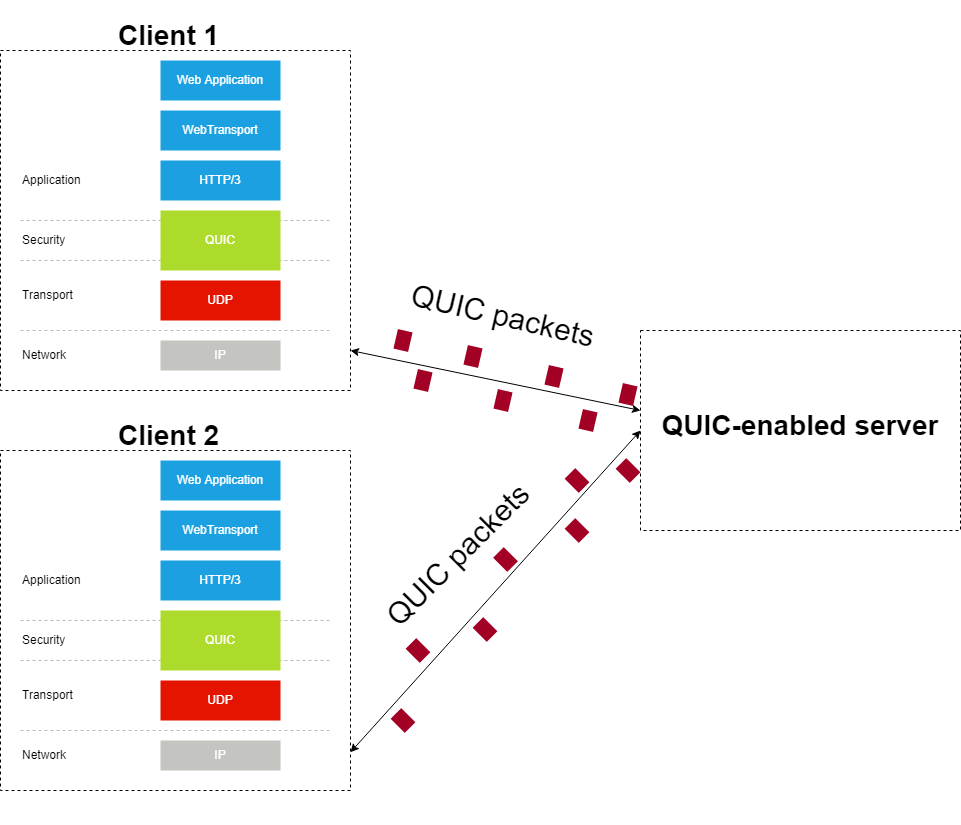
\includegraphics[width=0.7\columnwidth]{images/webtransport build diagram.png}
	\caption{System Diagram for WebTransport builds.}
    \label{wt_systemdiagram}
\end{figure}

On the left side of this diagram, we can see our two clients - each of these are a JavaScript web page running on Google Chrome browser windows. On the right side, we can see our QUIC-enabled server - this shall receive data from each client and forward this data to the other client. We shall explore several existing QUIC server implementations written in different languages whilst developing this server.

The general working pattern of our builds is simple. Clients will establish a connection to the server, transmit data and be ready to receive data - once both clients are connected, the server shall forward received data to each client in order to establish an information flow similar to the one illustrated in Figure \ref{wt_systemdiagram}. 

In Figure \ref{wt_systemdiagram}, the bidirectional arrows between each client and server represent what will either be WebTransport's streams implementation or its datagrams implementation. The diagram represents both builds and the general workflow of both is the same - the only difference is what the QUIC packets will be sent via.

We shall now outline high-level overviews of how the data will actually be sent and received by the WebTransport clients. There is a significant amount of shared functionality between the Datagrams and Streams builds, so this shall be covered first. Specifically, the two builds send data in almost the same way. After this, we shall diverge and talk about the design choices unique to each build.

\subsection{Sending Data - Datagrams and Streams Builds}

Firstly, our client requests and accesses the user's camera. Then, at regular intervals, the client shall send data generated from the user's media feed to the server. This data will be a frame of image data and some arbitrary amount of audio data. Then, the client shall encode this data into chunks and send these chunks as packets until a full frame of video data and the full amount of audio data have been transmitted. This is illustrated in Figure \ref{wt_sending data} - here, a chunk of data (at an arbitrary position for illustration purposes) is taken from our frame of image data, packaged into a packet and transmitted to the server via either WebTransport's streams or datagrams implementation.

\begin{figure}[h]
    \centering
    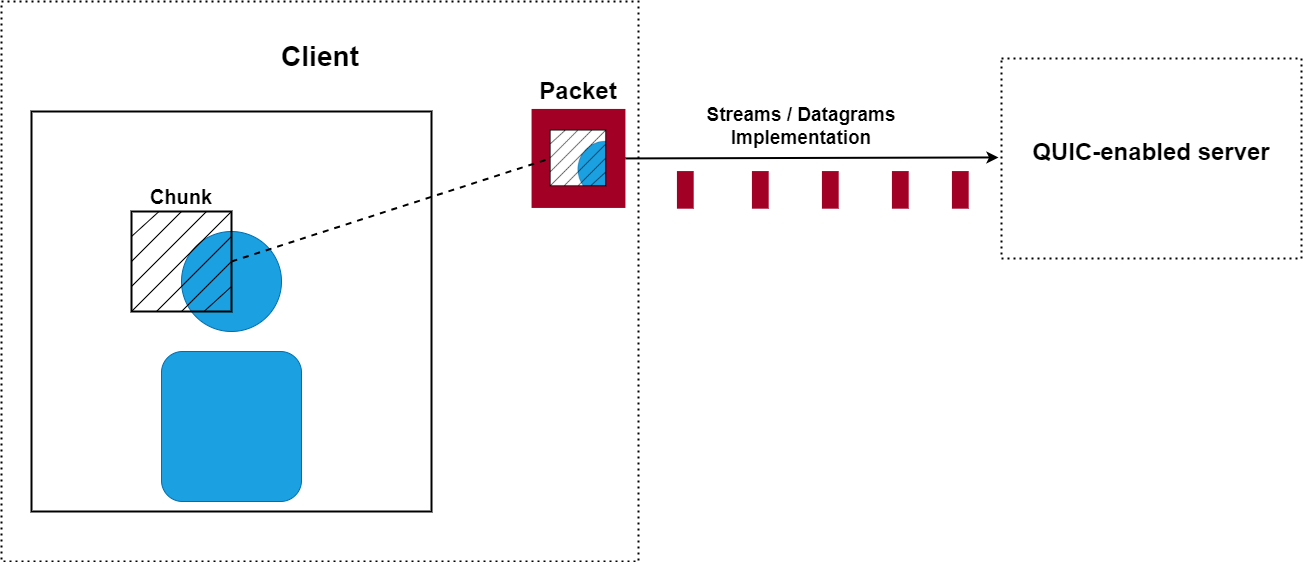
\includegraphics[width=0.9\linewidth]{images/sending data.png}
	\caption{An illustration of how WebTransport clients encode and transmit video data.}
    \label{wt_sending data}
\end{figure}

Additionally, header values shall prelude the data in these packets - specifically, these header values shall be a user ID, a packet sequence number, a frame number, a timestamp and an integer value (we shall call this eof) indicating whether the frame and chunk has been fully sent. During and after this process, relevant header data shall be updated continuously; specifically, the sequence number increases as packets send, the frame number increases as frames send and the eof sets to 1 when a frame and chunk have finished sending. Meanwhile, at the rate of the specified regular interval, more frames and audio data will be getting queued to be decomposed and sent. This process is applicable to sending data via both datagrams and streams.

Whilst this is occurring, the server shall be receiving this data and passing it on to the other connections in the session. We shall now examine how the WebTransport clients handle received data.

\subsection{Receiving Data}
The client shall constantly be waiting to read data. When data is received, the way it is handled depends on the specific build - the builds are similar, but the Datagrams build has a lot of extended functionality to handle the disordered and unreliable nature of datagrams. We shall now examine how data is received in each build, starting with the Streams build.
\hfill\\
\subsubsection{Receiving Data - Streams Build}
\hfill\\
The Streams build will handle receiving data more simply than the Datagrams build. 
The client will first check if a maintained buffer offset variable in addition to the size of the received data is greater than the size of the received frame. If it is, the received data will be cut down so that only the data that is necessary to receive a full frame is read. The leftover data will be stored in another variable. This will only happen when the last necessary packet to receive a full frame is read and prevents unnecessary data being processed. 

Then, the client shall add the received data to a buffer at a specified offset value. This offset value will then update to accommodate for the new data in the buffer. 

\begin{figure}[h]
    \centering
    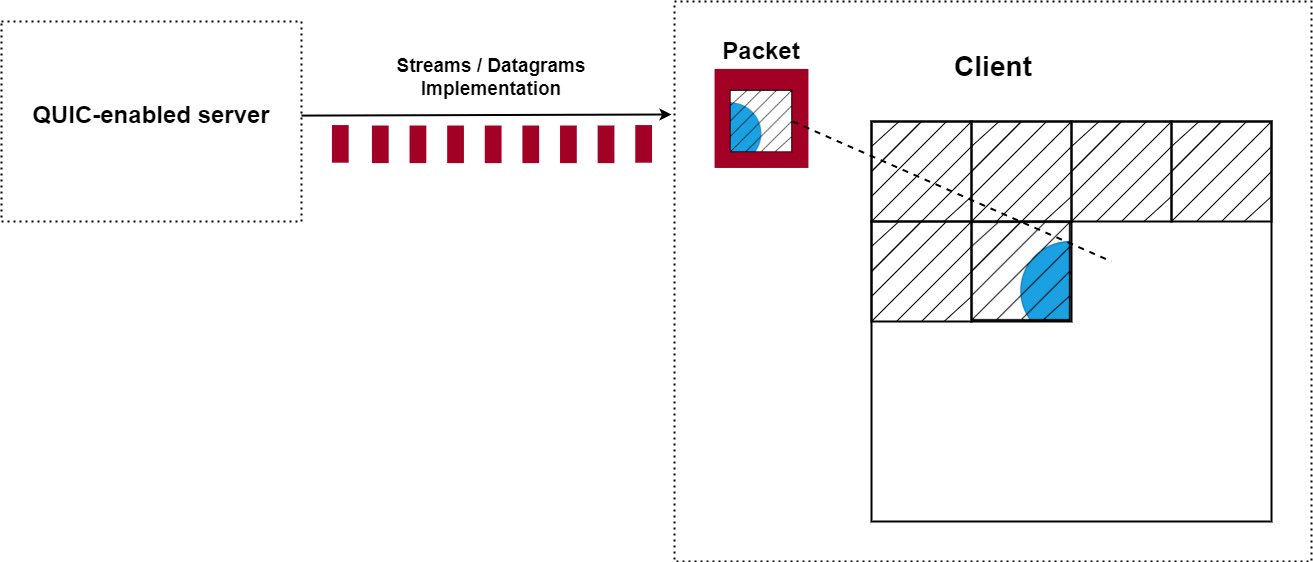
\includegraphics[width=1\linewidth]{images/receiving data.png}
	\caption{An illustration of how WebTransport clients receive video data and builds up a frame.}
    \label{wt_receive data}
\end{figure}


The client shall repeat this process until the buffer offset is equal to the size of the received frame. Then, the client will render this complete frame and the buffer offset and buffer shall return to their first states. An illustration of how a frame is built up can be seen in Figure \ref{wt_receive data}. 

Finally, the leftover data (which belongs to the next frame) is added to the buffer and the whole process repeats. This is done to ensure that no received data is wasted. We can operate this way because we know that all data will be received due to the reliable nature of streams. A similar process shall be undertaken for audio and chat data.

% \todo{is this too technical - should details of e.g. buffer offsets and leftover data belong in implementation?}

We shall now examine how the Datagrams build receives data.
\hfill\\
\subsubsection{Receiving Data - Datagrams Build}
\hfill\\
The Datagrams build operates in the same way as the Streams build, but has some additional complexity that handles packet loss and reordering.
The client shall extract the headers from the received packet - this is achievable as datagrams, unlike streams, preserve message boundaries.The client shall use these headers to gain knowledge on what frame number the packets currently being processed are from - this information shall be utilised to reorder packets and create some sort of "timeout" for frames that take too long to have data be retransmitted. To elaborate, if, for example, "Frame 8" takes too long to have the last third of its data be transmitted (thus disrupting the user experience), the client shall know to render what they have of "Frame 8" and move on to queued data from "Frame 9". An illustration of this can be seen in Figure \ref{wt_design_latepackets}.

\begin{figure}[h]
    \centering
    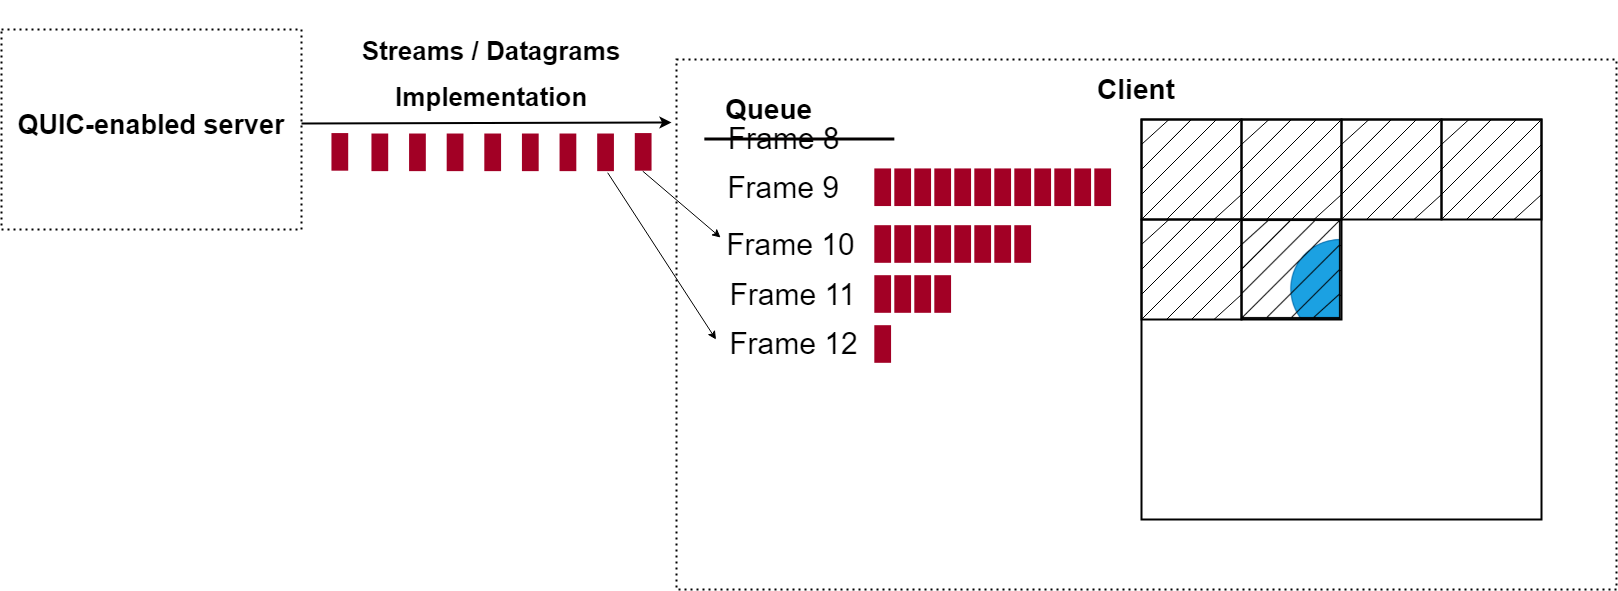
\includegraphics[width=1\linewidth]{images/late packets.png}
	\caption{An illustration of how WebTransport clients discard packets of a certain frame after an arbitrary timeout.}
    \label{wt_design_latepackets}
\end{figure}

The client shall continue building a frame even when data is lost. It does this by altering the buffer offset to account for where the lost data should have been inserted into the buffer. An illustration of this can be seen in Figure \ref{wt_design_shifteddata}.

\begin{figure}[h]
    \centering
    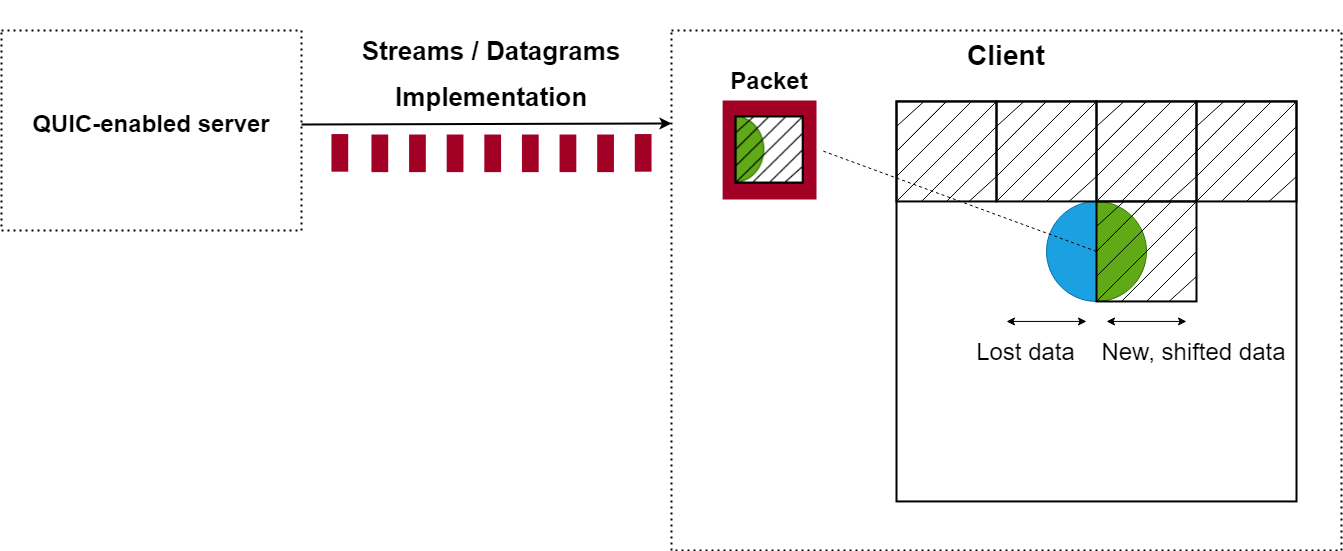
\includegraphics[width=1\linewidth]{images/shifted data.png}
	\caption{An illustration of how WebTransport clients shift received data to deal with lost packets.}
    \label{wt_design_shifteddata}
\end{figure}

This combination of techniques to handle loss and reordering should prove as adequate measures for combatting the unreliable and disordered nature of datagrams. Chat and audio data shall be handled similarly, although chat data particularly will not require such complex handling.

This summarises how the WebTransport builds shall send, receive and display data. We shall now examine how the WebRTC build shall work.

\section{WebRTC - Process}
Developing the WebRTC build shall be a much more high-level and simple experience, utilising available libraries and extensions to WebRTC as well as existing online tutorials. My reasoning for this is that a factor in the evaluation of WebTransport's potential is the developer's experience - WebTransport may facilitate more effective video transfer, but extra development overhead may make it undesirable for software developers to actually make use of it. Because of this, I shall make use of existing libraries and tutorial resources to allow for comparison between the development experiences of projects utilising WebRTC and WebTransport.

% \subsection{PeerJS}
% From a developer's perspective, PeerJS greatly simplifies WebRTC's connection establishment process - PeerJS allows developers to create a peer-to-peer media stream connection utilising nothing but this ID. This library provides a JavaScript API. In the application, we shall generate this unique ID and use it to connect to our peer.

% \subsection{socket.io}
% socket.io is a JavaScript library that enables real-time, bi-directional communication between web clients and servers. socket.io utilises WebSockets - this is an established API that allows for reliable, ordered and untimely data transfer between a client and a server in a single stream. WebSockets is similar to WebTransport, but is not as customisable, suffers from head-of-line blocking and transports data via TCP rather than QUIC \cite{websockets_mozilla_docs}, thus making it generally unsuitable for media transfer.

% In our application, we shall utilise socket.io to facilitate the communications relating to setting up "rooms" for users to join. These rooms will again be based on a unique ID generated by the application. 

The application shall set up a server that facilitates communication of logic relating to "rooms". These rooms will act as sessions for different clients to exist in - they shall be created when a client starts a new session and automatically generates a unique ID that acts as the "room ID". Our reasoning for including rooms is that it shall showcase the widely available and open source additional functionality in WebRTC projects (something not yet seen with WebTransport). Once routed to the correct room, a client shall have another unique ID generated to correspond to their "user ID". The client shall then have the user's media feed accessed and displayed. Once a second client connections, the clients shall establish a peer-to-peer connection to each other and media data shall be exchanged. Each client shall receive the others' media data and this will be displayed alongside their own media feed. Chat data shall be sent utilising WebRTC's data channel, and media data shall be sent via WebRTC's media channel.

\hfill{} \\
Thus concludes all of our designs. Due to the relative lack of existing research on the subject area, we recognise that it is hard to determine how many of these builds we will be able to implement within the timescale of the project. This is because it is unknown how much difficulty we will have with development, particularly for the WebTransport builds. However, we decided that we would rather design too many builds to evaluate than too little, and implement as many as we can in order of importance.


% How is this problem to be approached, without reference to specific implementation details? 
% \section{Guidance}
% Design should cover the abstract design in such a way that someone else might be able to do what you did, 
% but with a different language or library or tool. This might include overall system architecture diagrams,
% user interface designs (wireframes/personas/etc.), protocol specifications, algorithms, data set design choices,
% among others. Specific languages, technical choices, libraries and such like should not usually appear in the design. These are implementation details.


%==================================================================================================================================